\documentclass{standalone}
\usepackage{tikz}
\usetikzlibrary{arrows.meta}
\begin{document}
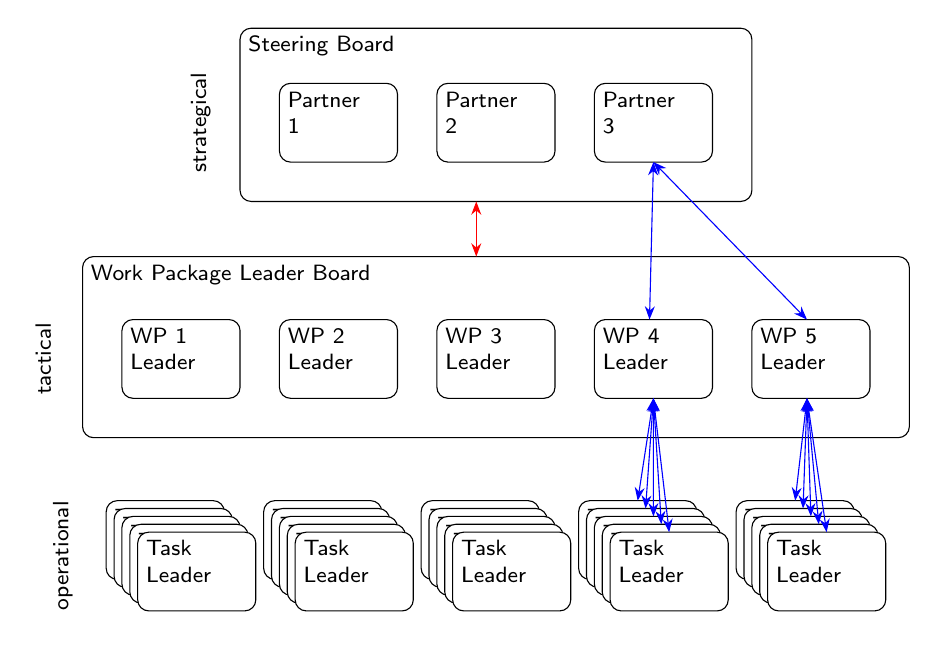
\begin{tikzpicture}[every node/.style={font=\sffamily}]
    \footnotesize
    \tikzset{>=Stealth}
    \draw[rounded corners] (-1.5,3.2) node[below right] {Steering Board} rectangle (5,1) ;

     \foreach \i in {1,2,3}
        \draw[rounded corners] (-3+2*\i,2.5) node[below right] {\parbox{1.5cm}{Partner\\ \i}} rectangle (-1.5+2*\i,1.5) ;
    
    \draw[rounded corners] (-3.5,0.3) node[below right] {Work Package Leader Board} rectangle (7,-2) ;
    \foreach \i in {1,...,5}
        \draw[rounded corners] (-5+2*\i,-0.5) node[below right] {\parbox{1.5cm}{WP~\i\\ Leader}} rectangle (-4+2*\i+0.5,-1.5) ;

        % \draw[rounded corners,fill=gray] (-4,-3.5) node[below right] {} rectangle (7,-6) ;
    
    \foreach \i in {1,...,5}
        \foreach \ii in {-0.2,-0.1,...,0.2}{ 
            \draw[rounded corners,fill=white] (-5+2*\i+\ii,-3-\ii) node[below right] {\parbox{1.5cm}{Task\\ Leader}} rectangle (-4+2*\i+\ii+0.5,-4-\ii);
            }            
    \foreach \i in {4}
        \foreach \ii in {-0.2,-0.1,...,0.2}{ 
            \draw[blue,<->] (3.75,-1.5) -- (-4.5+2*\i+\ii+0.25,-3-\ii);
            }            
    \foreach \i in {5}
        \foreach \ii in {-0.2,-0.1,...,0.2}{ 
            \draw[blue,<->] (5.7,-1.5) -- (-4.5+2*\i+\ii+0.25,-3-\ii);
            }            

    \draw[red,<->] (1.5,1) -- (1.5,0.3);

    \draw[blue,<->] (3.75,1.5) -- (3.7,-0.5);
    \draw[blue,<->] (3.75,1.5) -- (5.7,-0.5);

    \node[rotate=90] at (-2, 2) {strategical};
    \node[rotate=90] at (-4, -1) {tactical};
    \node[rotate=90] at (-3.75, -3.5) {operational};
    
    \end{tikzpicture}
\end{document}